Consider the following feedback control system
\begin{center}
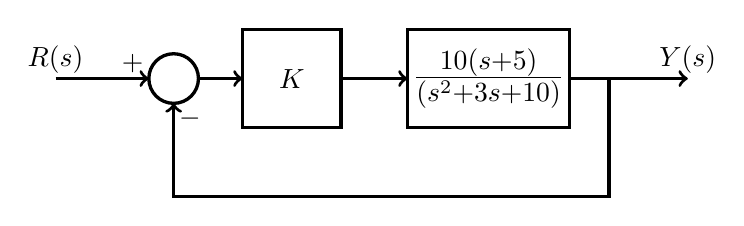
\begin{tikzpicture}[scale=1,inner sep=0pt,outer sep=0pt,very thick,
sysblock/.style={draw,rectangle,inner sep=2pt,minimum width=1.25cm,minimum height=1.25cm,very thick}]
\draw (2,0) node[draw,circle] (sum1) {$\rule{0pt}{18pt}$};
\draw (3.5,0) node[sysblock] (K) {$ K$};
\draw (6,0) node[sysblock] (G) {\Large $\frac{10(s+5)}{(s^2+3s+10)}$};
\draw[->] (.5,0) node[above=2pt] {$R(s)$} -- (sum1.180) node[above left=2pt] {$+$};
\draw[->] (sum1.0) --  (K);
\draw[->] (K) -- (G);
\draw[->] (G.0) -- ++(1.5,0) node[above=2pt] {$Y(s)$};
\draw[->] (G.0) ++(0.5,0) -- ++(0,-1.5) -| (sum1.-90) node[below right=2pt] {$-$};
\end{tikzpicture}
\end{center}
\begin{enumerate}[(a)]
\item Mark the open loop poles and zero on the complex plane using the usual 'x' and 'o' notation.
\item Compute the closed-loop poles for the following values of $K$ and mark them as small squares on the complex plane: $K = {0.1, 0.4, 0.8, 1.2, 1.5, 1.59, 1.6, 2}$. Note on the plot the gain value associated with each pair of closed-loop poles. (\textit{Hint: you may find \textsc{Matlab}'s \texttt{feedback} and \texttt{pole} commands helpful.})
\item Roughly sketch the locus by connecting the marks. Remember that loci start at open loop poles ($K=0$), move through closed-loop poles as $K$ grows, and end at open loop zeros or infinity.
\item Verify your loci by using the \texttt{rlocus} command in \textsc{Matlab}. Note that this kind of circular loci is common but not easy to sketch using the root locus rules of Lecture 20.
\end{enumerate}